% % % Set the style for this file:
\pagestyle{standard}

% % % Beginning of the chapter
\chapter{Thermograms calibration.}\label{chapter4}

	% % % Set the style for the first page:
	\thispagestyle{chapter-first-page}

	\section{Emissivity correction methods. }\label{section4.1}
		
		As the main source of discrepancies comes from the differences in emissivity, this is very often the starting point for IR image calibration. Almost all IR cameras can be set to a certain value of emissivity (usually set to 1.00 by default). If we knew the emissivity value of certain surface we could then enter that value into the IR camera software and the apparent temperature, i.e. temperature displayed by the IR camera, would be close to the real temperature. This is what we would call a “direct” emissivity correction method. It is of course the most simple but also the most uncommon way to correct an IR image for more complicated quantitative studies. On one side, we usually don’t know beforehand the emissivity value of the surface we want to measure and, on the other side, this method would only give us the correct temperature on the surface of known emissivity.
		
		There are also some other ways to calculate the emissivity of a surface. One of them consists in estimating the surface’s emissivity by using an alternative temperature measurement as reference. With that purpose, the following method can be used  \ref{ref11}, \ref{ref12}:
		
		\begin{enumerate}[label={\arabic*)}]
			\item Measure the surface temperature by an alternative method (thermocouple, known emissivity coating).
			\item Set the necessary measurement parameters (ambient temperature, RH, distance to target, ...) in the IR camera software as needed and the emissivity to 1.
			\item Point the IR camera to the target and select a region of interest (ROI).
			\item Modify the value of emissivity in the camera software until the apparent temperature in the selected ROI equals the one measured with the alternative method. This is the emissivity of the target surface.
			\item Repeat steps 2) to 4) as many times as necessary to minimize the measurement uncertainty.
		\end{enumerate}
		
		Using this approach a “global” IR image emissivity correction can be applied to get temperature values close to the real ones on the silicon surface. However, as mentioned before, this will only show accurate readings in those areas corresponding to the surface of estimated emissivity. The rest of the elements in the image that have different emissivity values might appear to have a complete different temperature of what they actually have. However, if we are not interested in the whole picture but just in one particular material in it, this simple method can be very useful. The problems begin when the surface of interest has relatively low emissivity. In such cases temperature estimation may not be very accurate because low emissivities are hard to estimate and small changes in their values can lead to large variations in the temperature measurements \ref{ref13}. In other words, the lower the emissivity of the surface, the bigger the uncertainty associated with it \ref{ref14}.
		
		Another approach consists in using a “relative” method exploiting the Equation \ref{eq1.16}. Let's imagine that we have two surfaces at the same temperature, then, if we apply Equation \ref{eq1.16} on the one that we know the emissivity value (e.g. black tape) and on the one we want to estimate it from (e.g. silicon surface) then we obtain:
		
		\begin{equation}\label{eq4.1}
		N^{BT}_{meas}(T_{BT})= R \cdot \bar{\varepsilon}_{BT} \cdot I_{1}(T_{BT}) + R \cdot [1- \bar{\varepsilon}_{BT}] \cdot I_{2}(T_{r})
		\end{equation}
		
		\begin{equation}\label{eq4.2}
		N^{Si}_{meas}(T_{BT})= R \cdot \bar{\varepsilon}_{Si} \cdot I_{1}(T_{BT}) + R \cdot [1- \bar{\varepsilon}_{Si}] \cdot I_{2}(T_{r})
		\end{equation}\bigskip
		
		Here $T_{BT}$ is the apparent (measured with the IR camera) temperatures of the black tape. Note that as the “real” temperature we have selected the apparent temperature of the black tape. We can do so since the black tape has high emissivity and therefore the IR camera should give accurate temperature readings without any further correction. Naturally we know that $N^{BT}_{meas}(T_{BT}) \neq N^{Si}_{meas}(T_{BT})$, however, we can use a small trick here: as the black tape has high emissivity, if we replace $T_{BT}$ in Equation \ref{eq4.1} with the apparent temperature of the silicon ($T_{Si}$) then $N^{BT}_{meas}(T_{Si}) = N^{Si}_{meas}(T_{BT})$. This is equivalent to say that we have measured a "real" temperature equal to $T_{Si}$ in then surface covered by black tape. After rearranging terms we obtain:
		
		\begin{equation}\label{eq4.3}
		\bar{\varepsilon}_{Si} = \bar{\varepsilon}_{BT} \cdot \frac{I_{1}(T_{Si}) - I_{2}(T_{r})}{I_{1}(T_{BT}) - I_{2}(T_{r})}
		\end{equation}\bigskip
		
		Note that this expression is invalid if the silicon surface is considerably transmissive, since we have neglected transmissivity for deriving Equation \ref{eq1.16}, and when the real temperature ($T_{BT}$) is close to $T_{r}$ in which case Equation \ref{eq4.3} does not hold anymore. This is known as the “black tape method” and, as the name indicates, consists in covering the surface of interest with a material of known emissivity (usually high emissivity) and use the direct correction method on the coated surface.
		
		For the Petal’s thermal study, parts of the silicon surface on both sides were covered with high emissivity black tape (Figure \ref{fig4.1}). The black tape used for this setup has an emissivity of 95\% and therefore the coated surface will behave almost like a blackbody. 
		
		\begin{figure}[ht!]
			\centering
			\captionsetup{justification=centering,margin=2cm}
			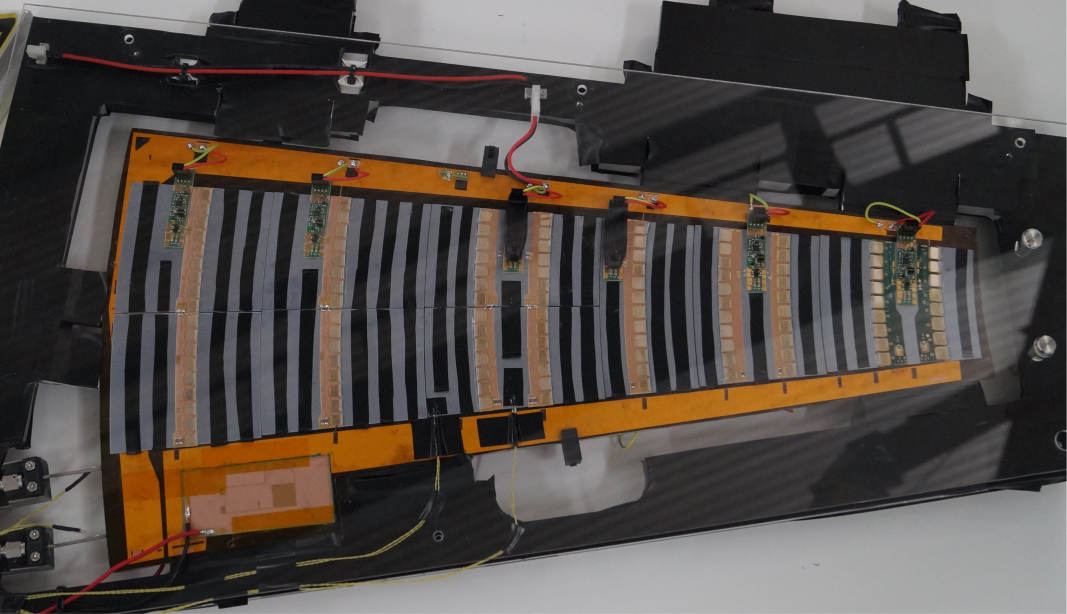
\includegraphics[scale=0.40]{Figures/Chapter04/ZebraPetal.jpg}
			\caption{Unpolished side of the “Zebra” petal covered with stripes of black tape of high emissivity.}\label{fig4.1}
		\end{figure}
		
		For our black taped petal (“zebra”), setting the IR camera emissivity to 0.95 (95\%) allows us to measure an apparent temperature very close to the real temperature. This is true if we assume that both the surface of interest and the black tape on top of it have reached thermodynamic equilibrium. Using the IRBIS software a set of over 560 measurement markers (ROIs) were created on the black tape strips to create a map of corrected temperatures. Additionally, a set of markers was created on the silicon surface right next to the corresponding black tape marker to be able to estimate the emissivity of the silicon using the black tape markers readings as the “real” temperature values. With this method we could perform calibrated temperature measurements on the petal’s silicon surface to be able to compare with FEA simulations (See section \ref{section4.4}). However, as it can be seen from the picture, we had to add adhesive material onto the silicon surface, which would be unacceptable during production stages for quality control. 
		
		Let’s now discuss another method, known as the “baseline image” method. Let's we assume that we have a thermogram of which we know the real temperature of all the pixels. That could be, for example, a thermogram of the petal at room temperature (Figure \ref{fig4.2}). The fact that we still see differences of temperature in the image even though everything is at the same temperature is evidence (to a first approximation) of the effect of the different emissivity values of the materials composing the petal. We call such image a baseline thermogram. The advantage of the baseline thermogram is that we know the real temperature of all the pixels beforehand and therefore we could use Equation \ref{eq1.16} to calculate the emissivity of each pixel. 
		
		\begin{figure}[ht!]
			\centering
			\captionsetup{justification=centering,margin=2cm}
			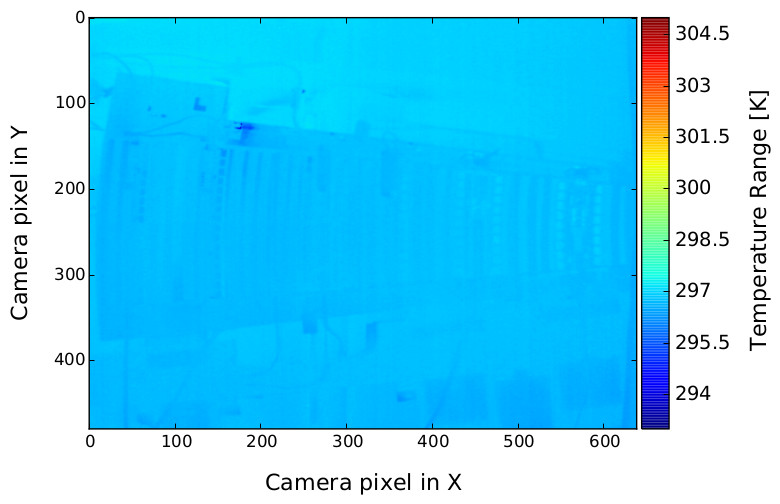
\includegraphics[scale=0.55]{Figures/Chapter04/thermo_Temp_201708091701_avg.jpg}
			\caption{Thermogram of the petal at room temperature (not powered and no CO$_{2}$ flushed in). Even though everything is at the same temperature, we still can see the shape of the petal.}\label{fig4.2}
		\end{figure}
		
		This method, however, presents an associated difficulty: if the baseline is at room temperature, it means that we can not use Equation \ref{eq1.16} directly to obtain emissivity but, instead, we can use it iteratively to estimate emissivity to some degree of accuracy. Of course this makes even worse the errors in the estimation of emissivity but it is the price to pay for not touching the petal. The other important disadvantage is that, in order to be able to extrapolate the values of emissivity calculated on the baseline image to other thermograms we must be sure that the camera does not move in between, otherwise the pixels won’t match anymore and the emissivity values would not be valid.
		
		Finally, we have also assumed that the emissivity does not depend on the surface temperature under the graybody approximation, which is not true in general. However, except for the case of selective emitters, emissivity is a very slowly-variating function of the surface’s temperature.
		
		The fact that the dummy silicon sensors in the front (unpolished) side of the petal are highly transmissive (See section \ref{section4.2}), together with the aforementioned difficulties, made it impossible\footnote{{\footnotesize This automatically invalidates Equation \ref{eq1.16} since transmission was ruled out in its derivation}} for us to use this emissivity correction method for the present study. Instead, the "zebra" petal approach, using the IRBIS set of ROI markers on the black tape strips was used for obtaining comparable results to FEA simulations.\bigskip
		
	\section{Silicon emissivity estimation.}\label{section4.2}	
		
		As shown in the previous section, one of the factors affecting the robustness of the measurements is the lack of “resolution” by using the black tape method, even though more than 560 markers were created (by hand) on the surface of the silicon sensors. This asks for more refined ways to measure the temperature of the silicon sensors. Furthermore, the black tape method is a quite invasive technique to use with the current prototype and for sure something to avoid during quality control with real petals.
		
		A good first approach would be to try to estimate the silicon emissivity and then use this value to correct globally the IR image. As mentioned in Section \ref{section4.1}, a “relative” method using the black tape markers measurements as temperature reference can be used to calculate the emissivity of the silicon next to them employing Equation \ref{eq4.3}. The IRBIS software also has an emissivity calculator, which reports the emissivity of a given pixel if we provide the real temperature of the pixel and the ambient temperature (apparent reflected temperature). However, as the calculations made within IRBIS are not known due to software copyright, we decided to use both methods and compare the results. As mentioned also in Section \ref{section4.1}, Equation \ref{eq4.3} will only work for opaque surfaces (not transmissive) and for surface temperatures well away from the apparent reflected temperature. For those reasons we performed this study on the unpolished side of the petal since the polished side is highly transmissive (Figure \ref{fig4.3}).
		
		Figure \ref{fig4.4} shows a profile plot (azimuthal projection) of one of the black tape strips in sensor R3 at the lowest temperature set-point (blue points). It is also included the temperature of a second set of markers in Silicon surface (red points) right next to each black tape marker. Both sets of temperature measurements were recorded with the IR camera. 
		
		We can see how both Silicon and black tape markers readings show two minima corresponding to the position through which the cooling pipe goes underneath the surface. We can also notice the large temperature difference between the Silicon and the black tape readings. This is mainly due to differences in emissivity: since the silicon surface has lower emissivity than black tape, the apparent temperature is higher. This apparent contradiction can be overcome if we think about it this way: since the black tape has higher emissivity, it is therefore better than the silicon at emitting the real (cold) temperature.
		In addition, the Silicon surface has relatively high reflectivity, which means that the camera also collects the ART more efficiently (See section \ref{section3.1}). As the ART is close to the ambient temperature inside the chamber, this would result in an additional contribution to the higher apparent temperature displayed for the Silicon.
		
		\begin{figure}[ht!]
			\centering
			\captionsetup{justification=centering,margin=2cm}
			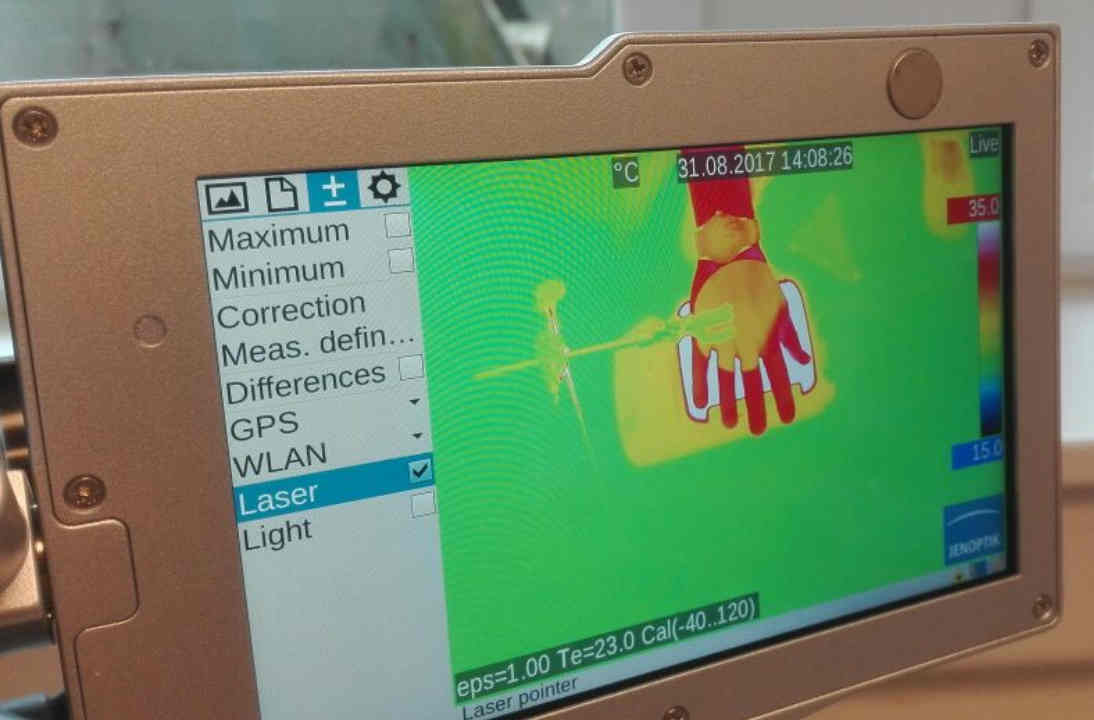
\includegraphics[scale=0.35]{Figures/Chapter04/HandTransmission.jpg}
			\caption{IR image (taken directly with the camera) of a circular piece of silicon wafer similar to the one glued on the polished side of the petal showing the high transmissivity properties of the silicon. Behind the silicon there is a heating plate at 150$^{\circ}$C and in between the experimenter’s hand (we can clearly see the fingers shape through the silicon).}\label{fig4.3}
		\end{figure}
		
		\begin{figure}[ht!]
			\centering
			\captionsetup{justification=centering,margin=2cm}
			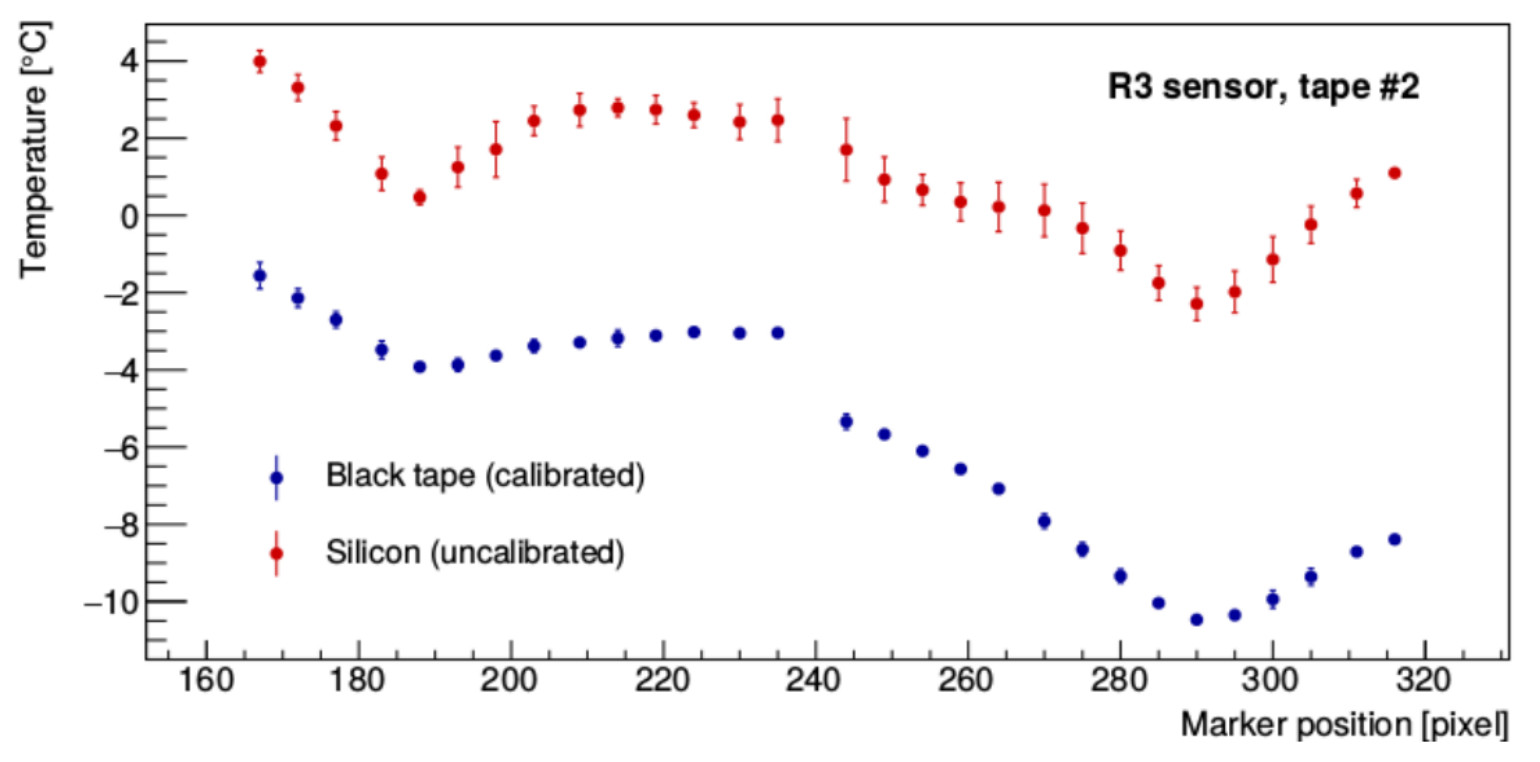
\includegraphics[scale=0.35]{Figures/Chapter04/R3Profile_Si_and_BT.jpg}
			\caption{Temperature profile plot of the second (middle) black tape strip in module R3 for the lowest temperature set-point.}\label{fig4.4}
		\end{figure}
		
		After applying Equation \ref{eq4.3} on each pair of silicon - black tape markers and using the IRBIS software emissivity calculation tool we obtained the results shown in Figure \ref{fig4.5}. As we can see the Equation \ref{eq4.3} estimations are in good agreement with the software outputs. 
		
		\begin{figure}[ht!]
			\centering
			\captionsetup{justification=centering,margin=2cm}
			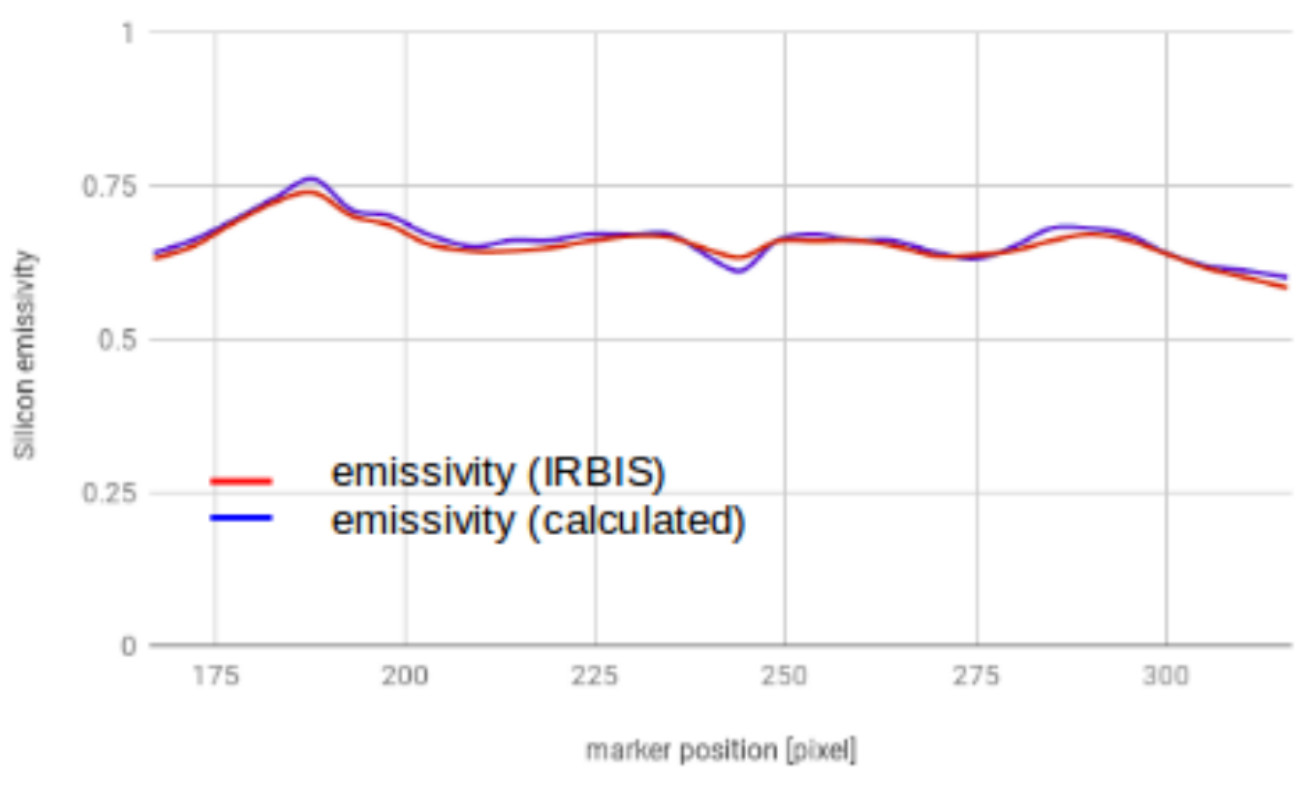
\includegraphics[scale=0.35]{Figures/Chapter04/SiliconEmissivityCalculatedVSIRBIS.jpg}
			\caption{Silicon emissivity calculated using Equation \ref{eq4.3} (blue line) and the emissivity calculation tool provided by the IR camera software (red line).}\label{fig4.5}
		\end{figure}
		
		The average emissivity is estimated to be around $0.66 \pm 0.07$. By entering this value in the IRBIS software we could correct “globally” the pixels temperature to yield silicon temperatures more close to the real values. However, this would worsen the calibration for the rest of the surfaces making their temperature values to shift greatly from the truth value.\bigskip
		
	\section{IR tests of the thermo-mechanical petal prototype.}\label{section4.3}
		
		For both thermal tests (one per side of the petal) the CO$_{2}$ pressure is varied in such a way that we go from room temperature to the lowest possible temperature and back again to room temperature in steps of 5$^{\circ}$C. After waiting long enough (~5 min) for the CO$_{2}$ pressure to stabilize at each set-point, the following data is recorded:
		
		\begin{enumerate}[label={\arabic*)}]
			\item Inlet/outlet pipes temperatures (using resistance thermometers - PT100).
			\item Temperature readings (PT100) on the silicon surface at each module (See Figure \ref{fig2.9}).
			\item CO$_{2}$ flow.
			\item Temperature of the CO$_{2}$ going in/out of the petal.
			\item Pressure of the CO$_{2}$ going into the petal and the difference to the pressure set-point.
			\item Ambient temperature and RH inside the chamber.
			\item Voltage/current readings from the power supply units.
		\end{enumerate}
		
		Also, the petal thermograms are recorded at each step following the method described in Section \ref{section2.3} at each step. Figure \ref{fig4.6} shows the cooling down and warming up profile of both sides of the petal. The measurements were taken at some selected places as indicated in the figure. Uncertainties of the IR measurements have not been included not to overload the plots but, as discussed also in Section \ref{section2.3}, the main source of uncertainty comes from the IR camera itself. 
		
		\begin{figure}[ht!]
			\centering
			\captionsetup{justification=centering,margin=0cm}
			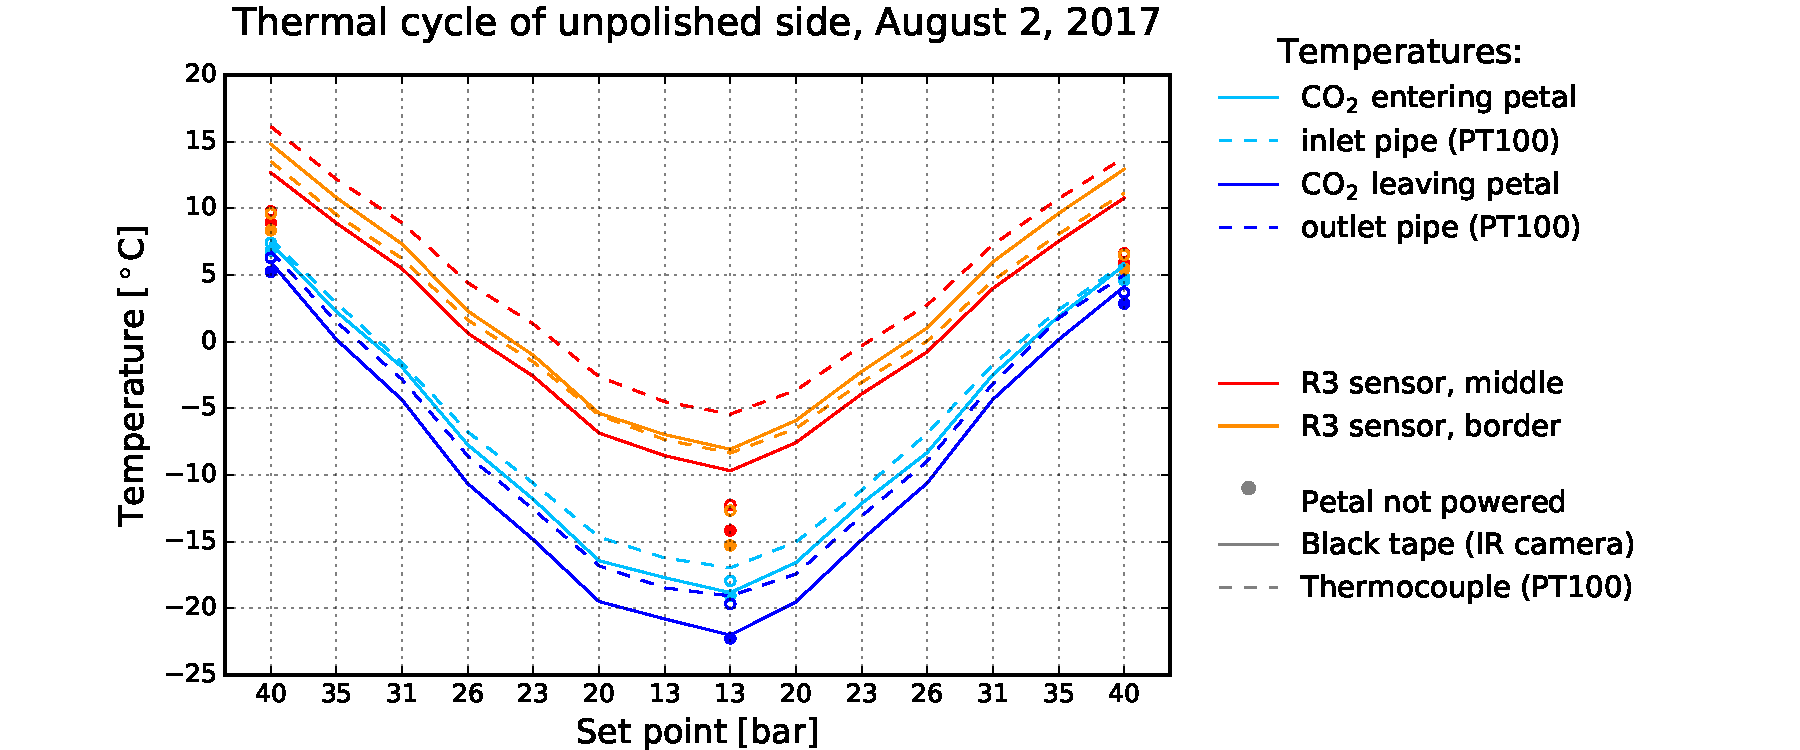
\includegraphics[scale=0.45]{Figures/Chapter04/unwrapped_cycle_2_201711121522.pdf}
			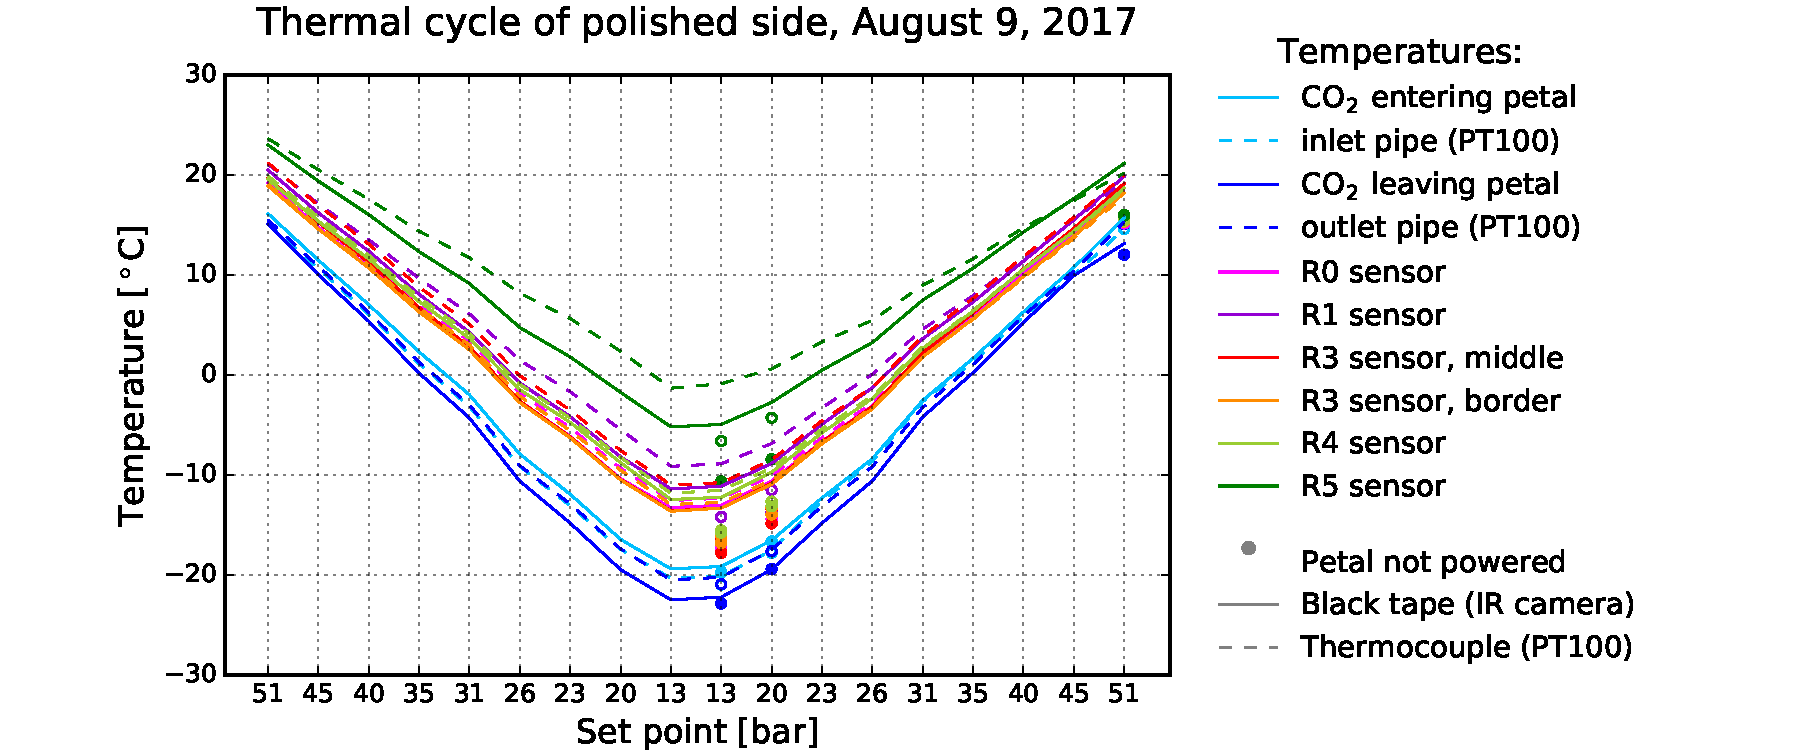
\includegraphics[scale=0.45]{Figures/Chapter04/unwrapped_cycle_9_201711121522.pdf}
			\caption{Temperature profiles for the thermal tests corresponding to the unpolished (front) and polished (back) sides. The dots represent set-points where the petal was not powered and the lines correspond to set-points with both sides of the petal powered. Solid lines and filled dots represent black tape readings with the IR camera (except CO$_{2}$ entering/leaving petal, given by the TRACI system) and dashed lines and hollow dots represent thermocouple values.}\label{fig4.6}
		\end{figure}
		
		As it can be seen, with the unpolished (polished) side test we were able to reach temperatures of around -18$^{\circ}$C (-20$^{\circ}$C). For both tests it is also notable that the returning CO$_{2}$ is colder, which is consistent with dual-phase cooling. We can also see that the PT100 thermocouple sensors report consistently higher temperatures than the TRACI sensors for both inlet and outlet pipes. This means that either we lost some cooling power due to thermal conductivity of the pipes, which is expected, or one of the sensors got incorrectly calibrated/placed. This situation is the opposite in the back side test with the inlet fluid temperature readings. In fact, for this test, the inlet PT100 accidentally broke and had to be re-glued, which might explain the difference from one test to the other in the inlet pipe while the outlet remained somewhat the same. This indicates that a correct manipulation of the thermocouple sensors is crucial to obtain good reliability on the measurements.
		
		Another interesting test that was performed is the comparison between the temperature reported by the IR camera using the black tape method and the temperature measured with an alternative method on the same surface (e.g. using PT100 thermocouples). In order to perform such a test, the additional PT100 sensors placed on the silicon surface were hold in position using the same high emissivity black tape used for the strips of the “Zebra” petal. For the front side test only two PT100s were used, as described in Section \ref{section2.4} while for the back side test four additional ones were placed. From Figure \ref{fig4.6} (top) we can see that the readings of the thermocouple and the IR camera are quite different for the sensor placed between the ASICs, possibly due to bad contact with the silicon surface (the sensors had to be placed very carefully not to damage the silicon). The other PT100 sensor, on the other hand, shows relatively good agreement with the IR camera measurement. The situation in the front side test improved a bit more, in general, for the lowest temperature set-point, specially in the R0, R3 (border) and R4, even though there are still large discrepancies (e.g. R5). As shown in the figure, all the profiles are quite symmetrical with respect to the lowest temperature point. However, it is also visible how most of the selected measurement points return to slightly lower temperature values than the initial ones. That does not necessarily means that the Silicon sensors are damaged after the tests, but instead, the TRACI system is the one that could remain altered in some way, specially since it is the CO$_{2}$ pressure the determining parameter in the temperature set-point.
		In any case, in order to properly determine how Silicon sensors respond to temperature changes, a more dedicated study involving several thermal cycles should be made. That is in fact one of the projected tests that the petal will have to go through in the future.\bigskip	

	\section{Comparison with FEA results.}\label{section4.4}	
	
		In order to compare the measured temperature values of the silicon sensors with the ones given by the FEA simulations, the black tape method was applied using IR camera readings from the black tape strips. Figure \ref{fig4.7} shows the thermograms at the lowest temperature achieved for the front and back side tests respectively. The tiny red squares correspond to the IRBIS measurement markers. Using linear interpolation in between each marker point corresponding to the black tape measurements, we were able to produce an isotherm map of the sensors as shown in figures \ref{fig4.8} (left) and \ref{fig4.9} (left). Figures \ref{fig4.8} (right) and \ref{fig4.9} (right) show the corresponding FEA simulation results \ref{ref15} for both front and back side tests respectively.
		
		\begin{figure}[ht!]
			\centering
			\captionsetup{justification=centering,margin=2cm}
			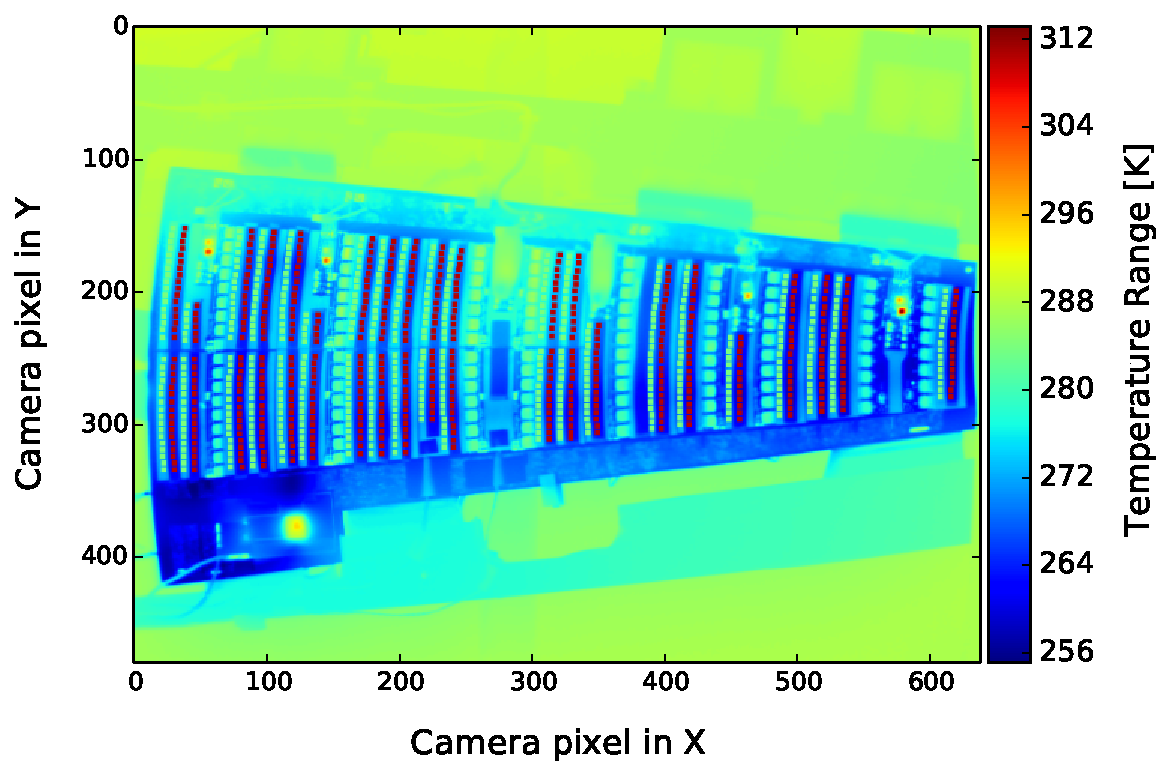
\includegraphics[scale=0.39]{Figures/Chapter04/thermo_Temp_20170803154926.pdf}
			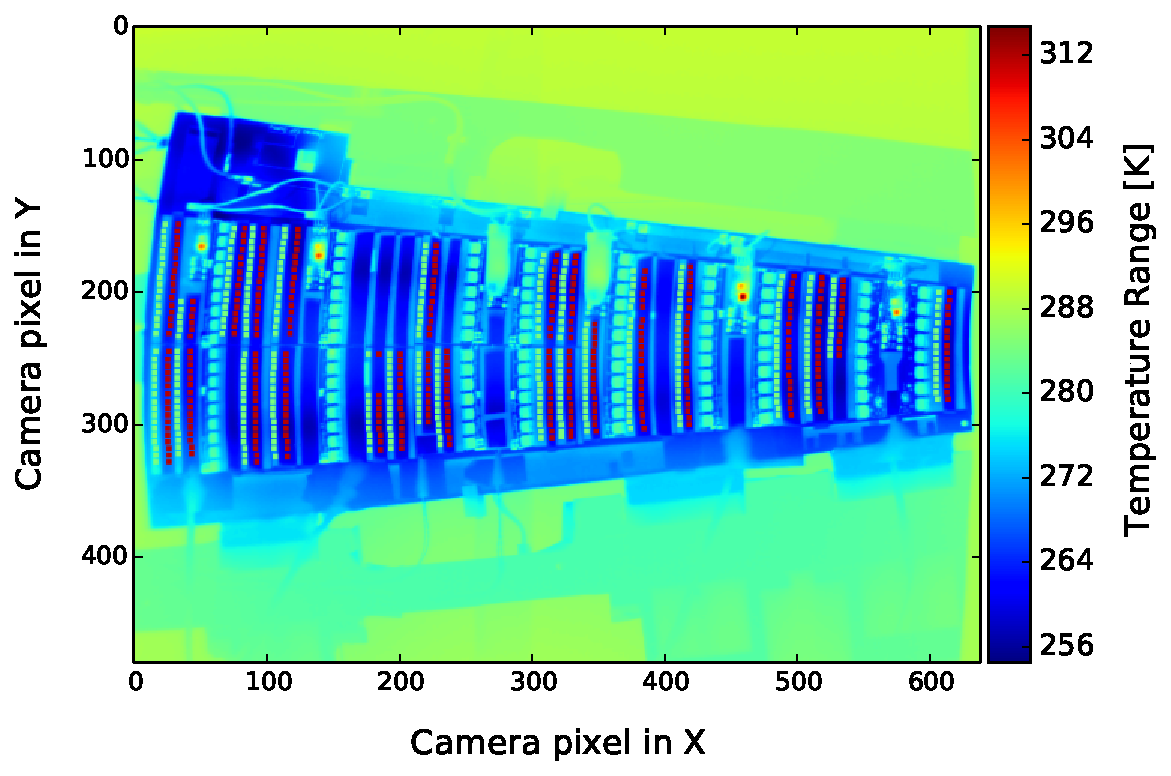
\includegraphics[scale=0.39]{Figures/Chapter04/thermo_Temp_201708101118_avg.pdf}
			\caption{Thermogram of the lowest temperature set-point in the front side test (left) and back side test (right) showing the IRBIS measurement areas (markers) defined on the black tape (red squares) and the corresponding silicon surface ones (blue squares).}\label{fig4.7}
		\end{figure}
		
		Before discussing the differences between the images in Figures \ref{fig4.8} and \ref{fig4.9}, we must say that this is to some extent an unfair comparison. While in FEA one have access to virtually every temperature point we are limited here by the number of markers and their uncertainty. Furthermore, the characteristics of the FEA model are not exactly compatible (e.g. power board thickness, cooling loop) and the thermal convection of the air surrounding the petal is very hard to model and is not accounted for in the FEA simulations. In fact, we know that the values of temperature reported by the markers near the R3 electronics (hottest point) is greatly influenced by the “halo” surrounding it, as discussed in Section \ref{section2.4}. In addition, in that precise region of the image, the linear interpolation tries to connect to distant measurement zones with no experimental point in between and thus, this area should not be very well described.
		
		In general (without paying too much attention to the temperature magnitudes), some similar features can be found between the experimental results and the FEA model. For instance, the hot spot at the corner of R5 is well reproduced in the FEA model for both the front and the back side of the petal. Additionally, the cold region corresponding to the path of the cooling pipe is quite similar. However, in places like R3 near the DC-DC converters, where the hottest point is expected to be, the agreement between IR measurements and simulations is worst due to the lack of experimental points in that area for a good linear interpolation.
	
		\begin{landscape}	
			\begin{figure}
				\centering
				\captionsetup{justification=centering,margin=0cm}
				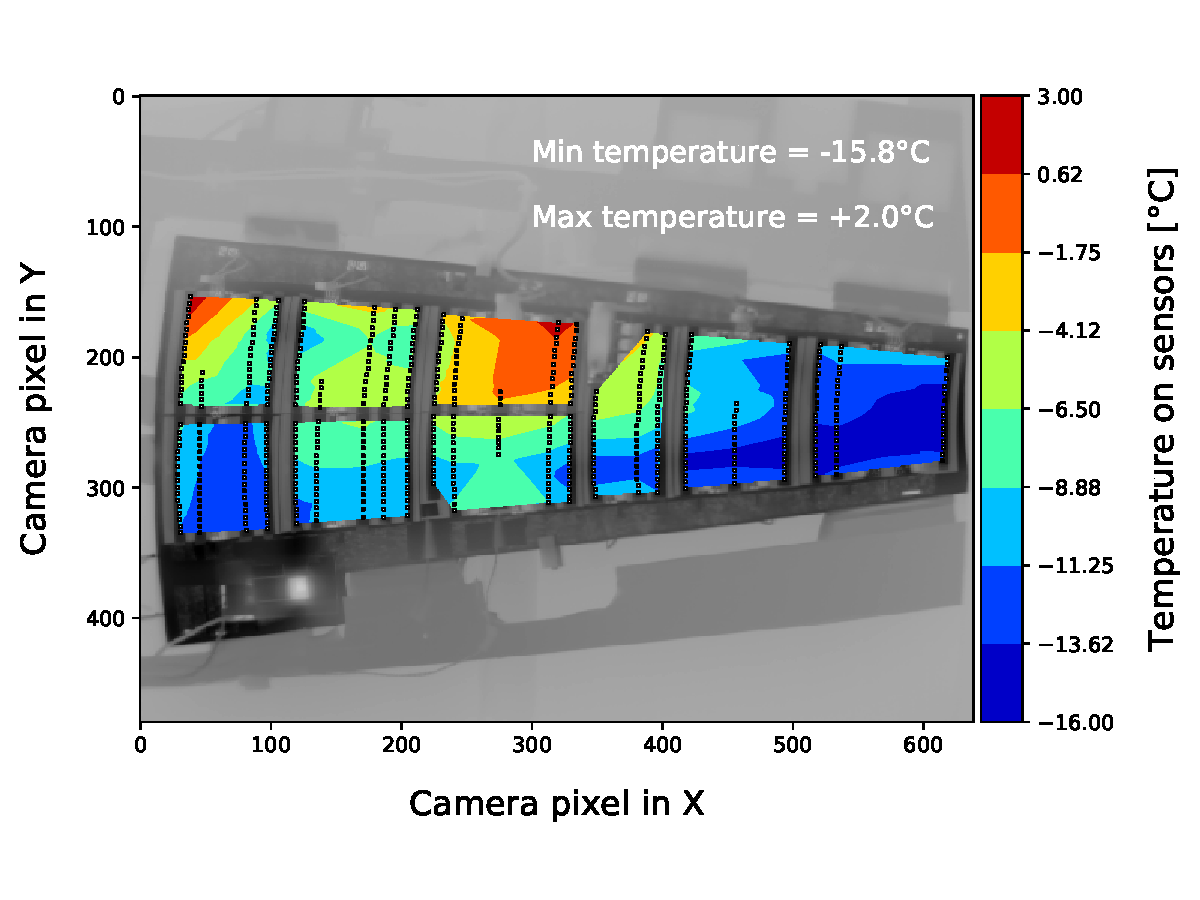
\includegraphics[scale=0.65]{Figures/Chapter04/thermogram_markers_2_201711271001.pdf}
				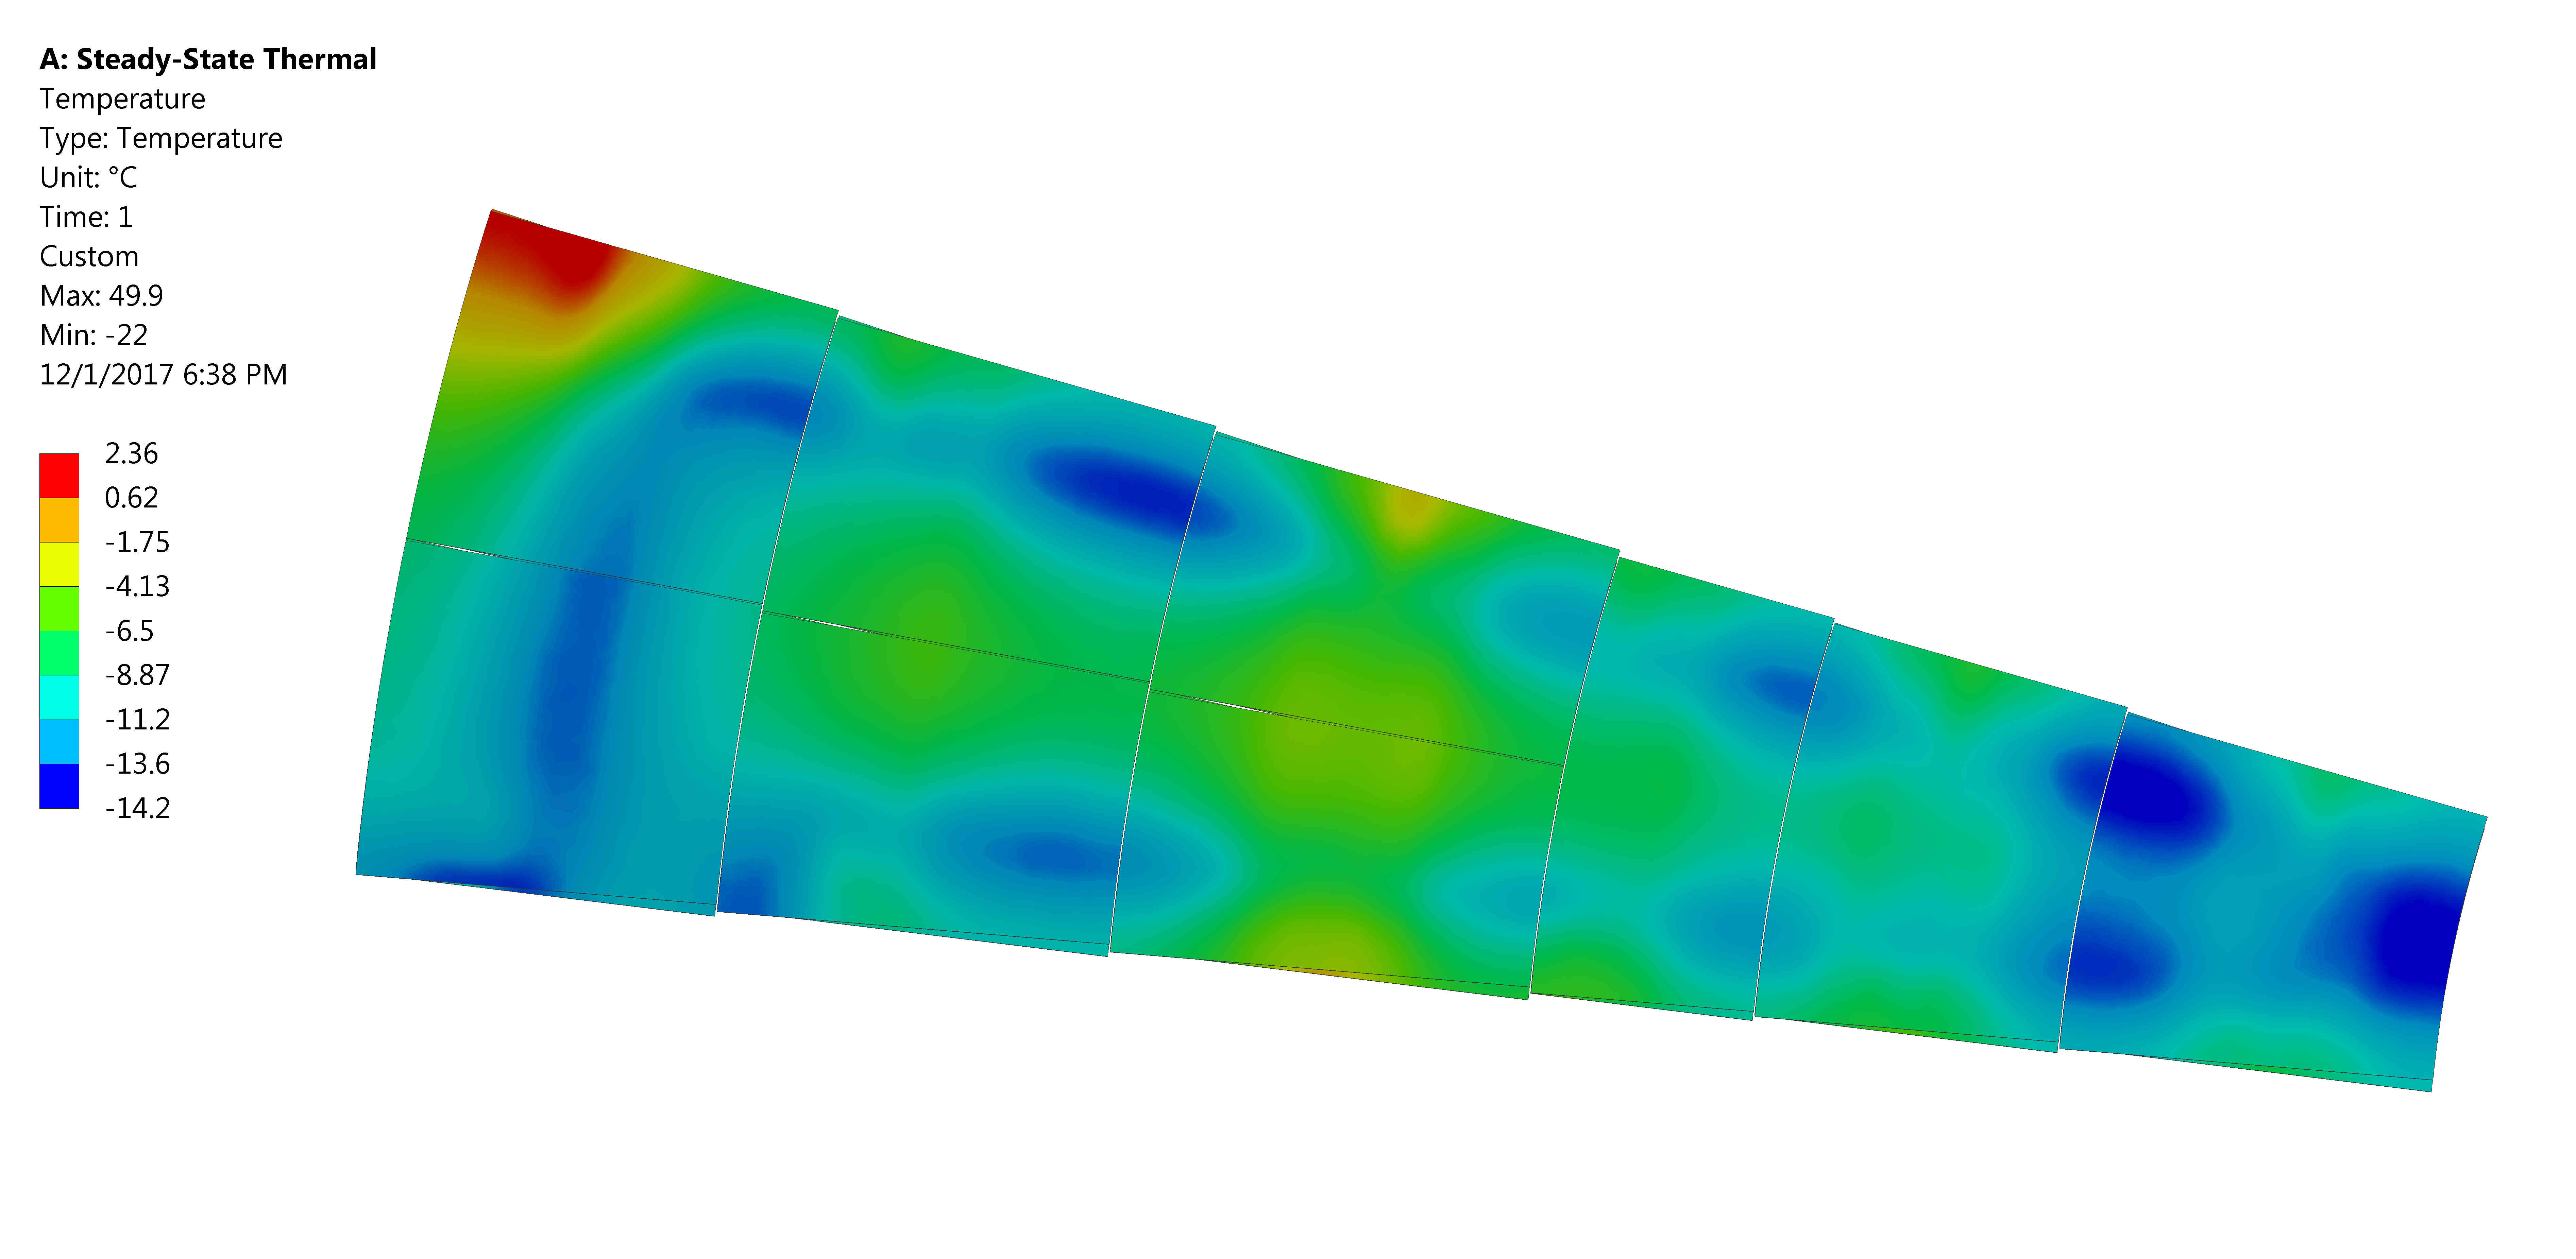
\includegraphics[scale=0.045]{Figures/Chapter04/FEA_thermogram_markers_2_201711271001.jpg}
				\caption{Isotherm contour for the thermal test of the front side of the petal (top) and the corresponding FEA simulation results (bottom). The temperatures displayed correspond to the petal silicon sensors.}\label{fig4.8}
			\end{figure}	
		\end{landscape}	
		
		\begin{landscape}		
			\begin{figure}
				\centering
				\captionsetup{justification=centering,margin=0cm}
				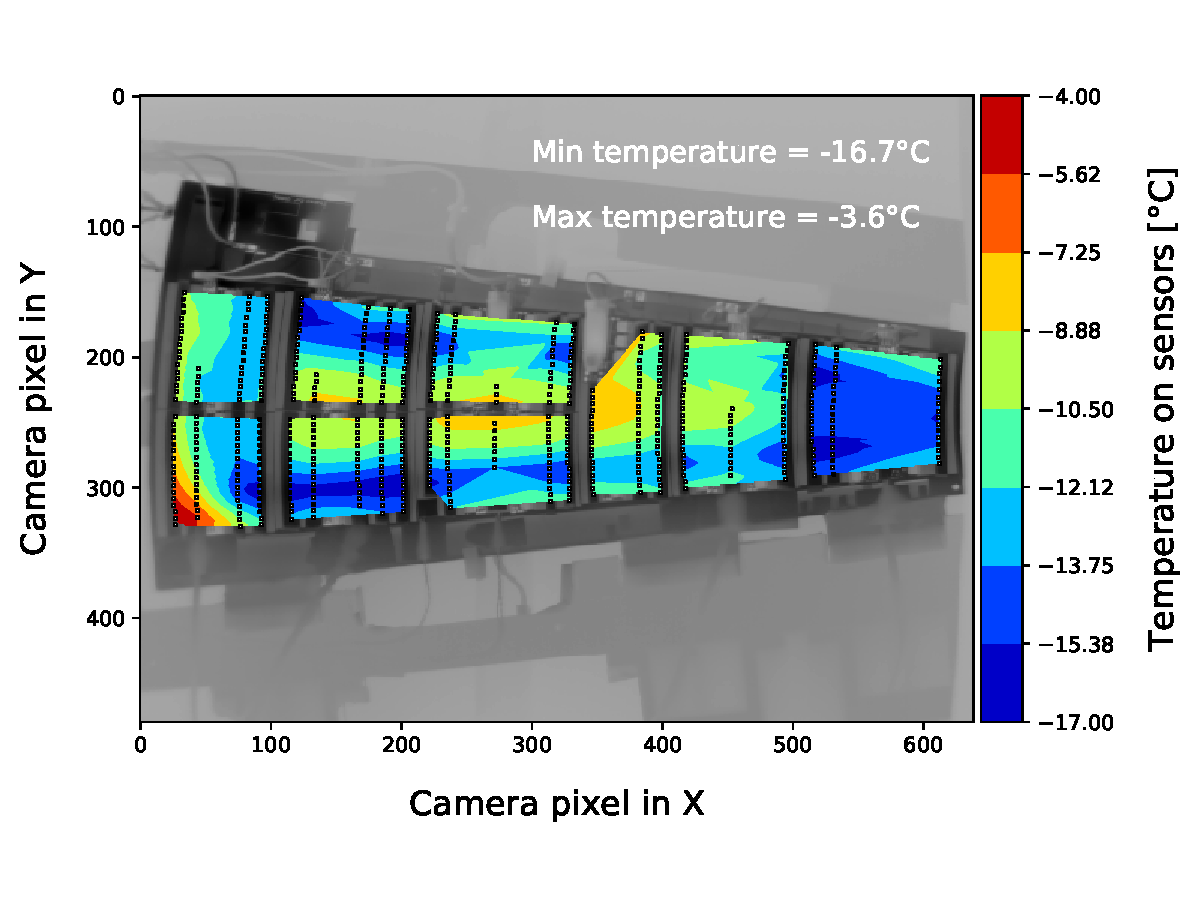
\includegraphics[scale=0.65]{Figures/Chapter04/thermogram_markers_9_201711271006.pdf}
				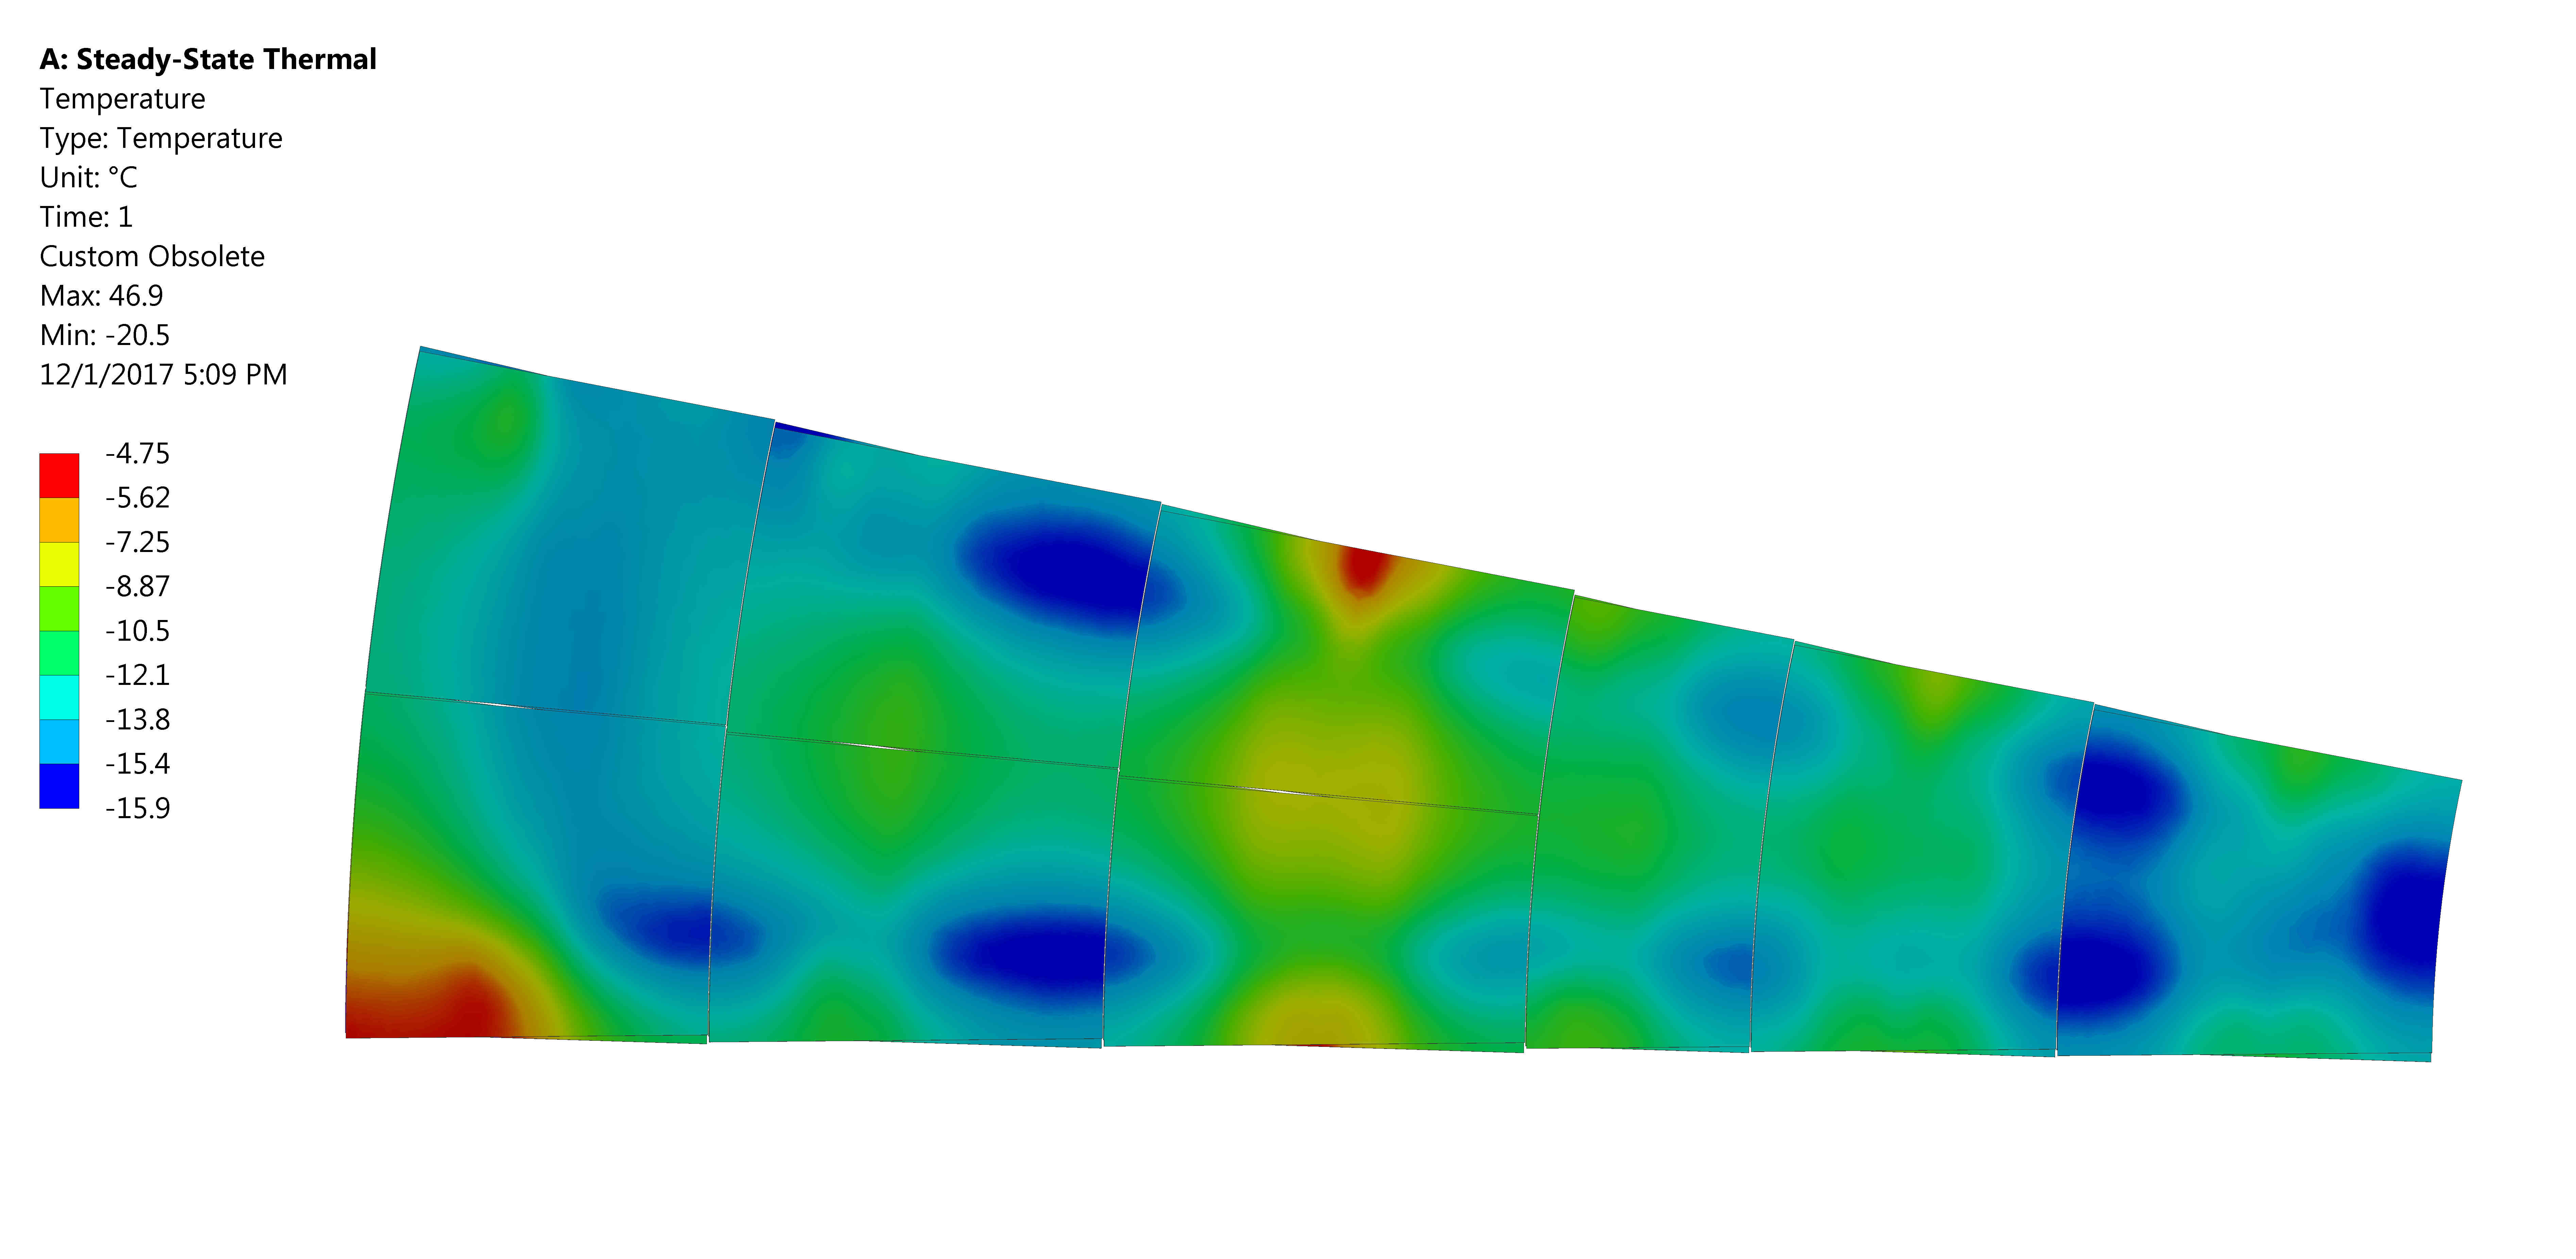
\includegraphics[scale=0.045]{Figures/Chapter04/FEA_thermogram_markers_9_201711271006.jpg}
				\caption{Isotherm contour for the thermal test of the back side of the petal (top) and the corresponding FEA simulation results (bottom). The temperatures displayed correspond to the petal silicon sensors.}\label{fig4.9}
			\end{figure}	
		\end{landscape}	